\section{Application}
\label{sec:app}


The Smartphone application was developed for Android using the Android Studio IDE. The Application is divided in two primary functional blocks, the Mock location Provider and the Google Maps Integrated Display, as can be visualised in figure \ref{fig:implementation}.

The Mock Location Provider is implemented as if it was a Location provider, such as GPS. The application functions works as a listener to a Location provider, in this case it listens to the Mock Provider that was implemented. By implementing the whole process of obtaining a location inside a service (the mock provider) , a new level of abstraction is added to the application. As such, whenever the application is signalled to obtain the user's current location, a request is made to the associated location provider and the application only need to listen for the answer that eventually arrives.

\begin{figure}
	\centering
		\includegraphics[width=0.5\linewidth]{4.Chapter/RequestLocation.png}
	\caption[Mock Location Provider Workflow]{Mock Location Provider Workflow}
	\label{fig:MockProvider}
\end{figure}

The Mock Location Provider incorporates the first three steps present in figure ~\ref{fig:MockProvider}, which will now be explored individually. The first step indicates the gathering of information of the surroundings of the user's device. When a request is made to the provider, a scan for nearby bluetooth low energy devices is made which will put the smartphone in a state of listening for incoming \ac{BLE} advertisement packets for half a second ( NEED TO VERIFY VALUE AND JUSTIFY, THERE WAS A PAPER ON THIS TODO). During this scanning period, each time a device is found, the advertisement is registered in a list, which have a duplication prevention mechanism implemented. Once the period is over, the provider has available a list of all the \ac{BLE} devices within range.   

The second step involves taking the created list of devices, obtain a server address and forward the same list to it. Once the first step is completed, the provider will analyse each entry at a time. For each device the provider will attempt to respond to the caught advertisement packet, resulting in a created connection.  Once the connection is created the provider asks for the available services of the paired device. Upon receiving an answer, the list of services is swoop while looking for the service with the wanted UUID. If the device doesn't have the UUID that the provider is looking for, it can assume that the paired \ac{BLE} is not a beacon of our system, as such the connection is terminated. When the provider identifies that the device has the system's UUID, it requests the device to provide the service's existent characteristics. The provider will receive a list composed of the service's characteristics and it will search in it for the system's characteristics UUID, the one which contains the device's server's address. This search has the objective of confirming that the service existent in this device is indeed the one that was implemented for the system and not a device with another service that happened to have the same UUID. For any service outside those that are documented in the Bluetooth Special Interest Group (SIG), who have a specific UUID attached to them, the UUID is generated randomly and as such there is a small chance of collision. Once the wanted characteristic is found, the provider requests the device to read its value and stores the received value in a list. This list will contain the servers of the devices that were found, and for each address there will be a list corresponding to each device , and their corresponding rssi values, from the same owner. In order to quicken the previously described process, the provider keeps in cache the most recent contacted devices. Before attempting a connection, the provider confirms that the device isn't found in cache and when finishing a process, the associated device is inserted into the cache.

When every device has been contacted, a voting system is actioned which will decide from the list of servers which one it will send the collected information to. The voting system uses an exponential function in order to attribute a weight to each server. %INSERT FUNCTION AND EXPLAINATION.

The voting system was implemented with the objective providing a thin security layer by allowing multiple devices of the same server to overcome a single attacker's device which happened to be close to the user. After obtaining each server's values, the one with the highest value is chosen and sent the list with all the devices. 

The Third step involves a simple client/server tcp interaction. The application starts off by formulating the message that it will later on send to the server, this message includes all pairs of device mac address and its associated rssi value captured by the application on the first step. Once the message is computed, the application attempts to create a connection with the server at the chosen address at the end of step two. With the connection established, the message is forwarded to the server and the application is put onto blocked state where it awaits for an answer. Upon arrival, the answer received is checked for valid location, its information is process and the connection is terminated. The information contained inside the received message, which was described in section ~\ref{sec:server}, is then processed into the adequate class capable of storing a geographic location and the same is broadcasted from the mock location provider to its listener. 



One of the current limitations of the android API that deals with \ac{BLE} is that the interface on the smartphone that is used to connect with a device has a fixed timeout time.  %MIGHT JUST NEED TO BE IMPROVED TODO


The Google Maps Integrated display is implemented using the Google Maps Android API. By using Google Maps it was possible to alleviate the weight on application since there wasn't need implement file transfer of indoor building's maps from each dedicated server to each request, which alleviated the servers as well since there was no need to store its associated building's maps on it. Managing the maps was something that was as well fortunately unnecessary and as such all these features were provided by google maps service. By making this development choice, the system as whole became closer to the desired generic approach while making possible for seamless transition between indoor/outdoor maps. The only imposed restriction is related to the addiction of new indoor maps onto the google maps, which is possible and well documented but dependent on a third party.

The Fourth step is called when the application receives a proper location from the request made onto the location provider. With the device's location known, a marker is placed on the map with the obtain coordinates (longitude, latitude), the camera is moved in order to be centralised on the position and fully displaying the indoor level map, and the menu visible on figure ~\ref{fig:AppMenu} is updated with the information that is bundled with the received location. In order to show the correct level on a multi level building, the "floor" information present in the menu is utilised. The API allows for obtaining a list of existent levels on which the maps' camera is focused and as such it's possible to find out to which level the provided location belongs and make so that the application shows it.

The pop-up menu was implemented to demonstrate the capacity of providing additional information associated with each location, be it geo-location taxonomy as it is currently implemented or possibly a description of the located room, an hyperlink of some sort or any other type of data that someone implemented this system would like to provide to its users.  

The final state of the implemented system can be visualised in figure ~\ref{fig:AppFocus} and figure ~\ref{fig:AppMenu}. The first displays the case of obtaining a location, where the marker has been placed and the camera zoomed

\begin{figure}
	\centering
		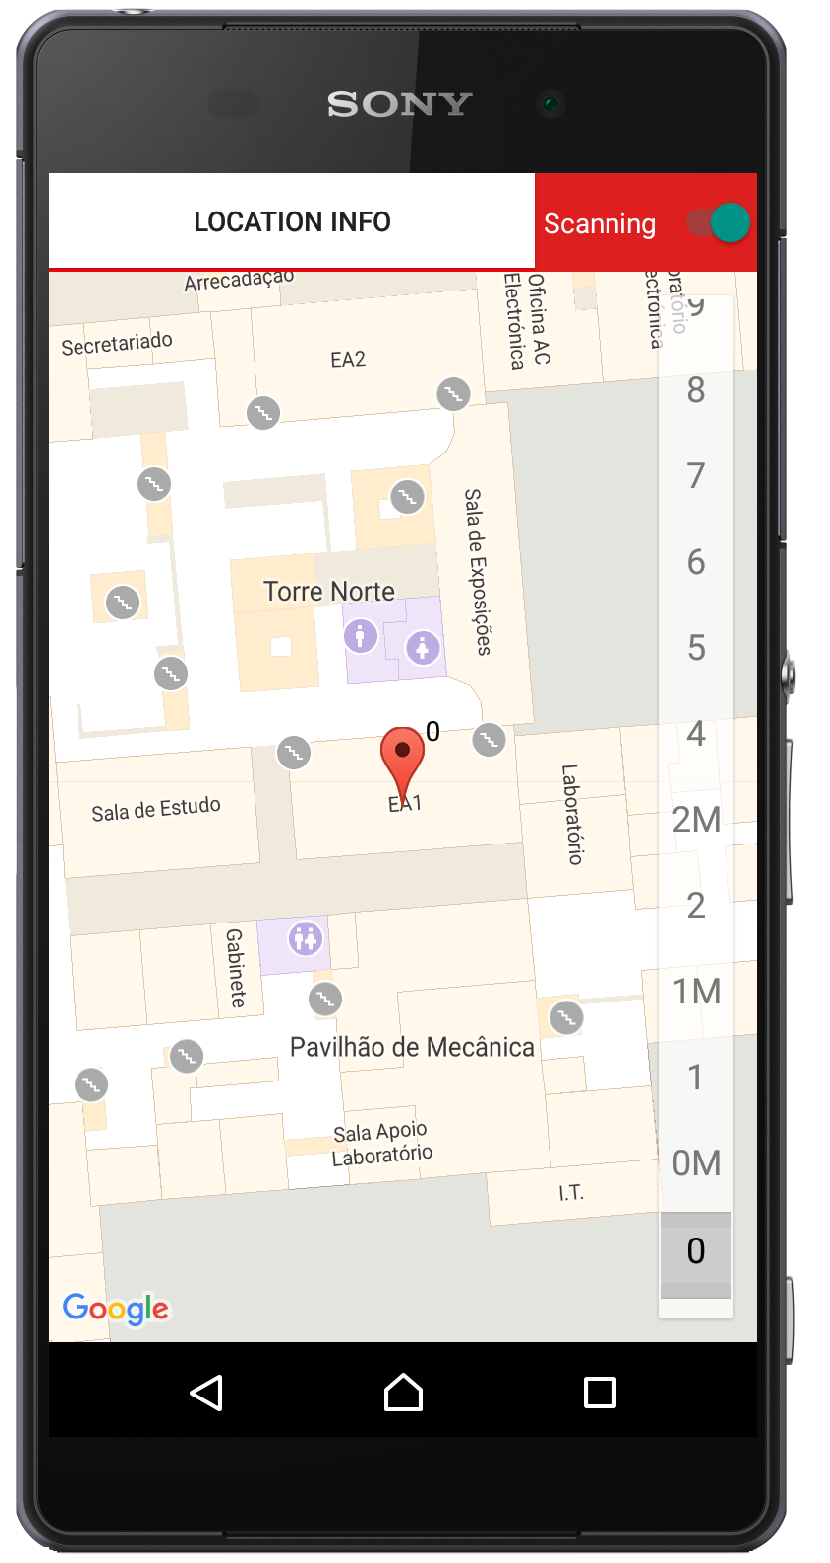
\includegraphics[width=0.5\linewidth]{4.Chapter/app_focused.png}
	\caption[Application screen showing a focused location on a room]{Application screen showing a focused location on a room}
	\label{fig:AppFocus}
\end{figure}

\begin{figure}
	\centering
		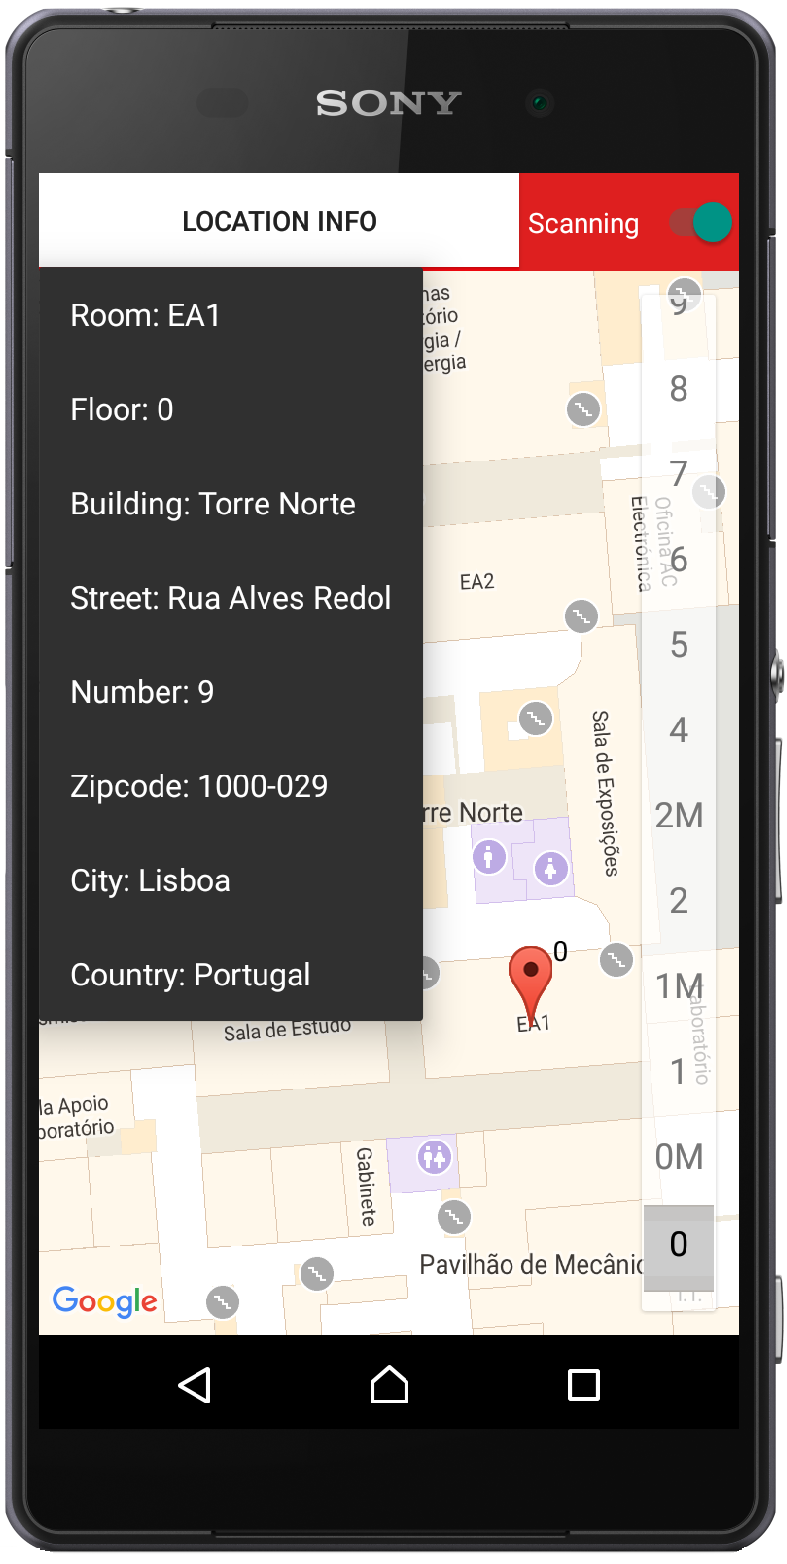
\includegraphics[width=0.5\linewidth]{4.Chapter/app_focused_menu.png}
	\caption[Application screen showing additional information of location]{Application screen showing additional information of location}
	\label{fig:AppMenu}
\end{figure}

